\chapter{Experiment 2: Effectiveness of Distractors}\label{chap:ex2}
This chapter consists of the Method, Results and Discussion components for Experiment 2. The experiment itself focuses on various effectiveness metrics for the developed redirected walking solution. 

\section{Method}
As part of developing the extension to the redirected walking toolkit, one of the implemented components was the AC2F algorithm. Since AC2F makes use of more predictive information compared to S2C, it would be interesting to see whether this provides a more effective solution when using distractors. As such, this experiment compares two different conditions. The first makes use of S2C only throughout an entire playthrough of Ensemble Retriever while the other uses S2C during walking and AC2F during the standing distractor battles. The redirection gains employed in this experiment are derived from the estimated thresholds in Chapter~\ref{chap:ex1}. This playthrough of Ensemble Retriever is also somewhat shorter than in Experiment 1, taking roughly 15-20 minutes instead of \textasciitilde30 minutes in hopes that it would make it easier to gather participants. The post-test questionnaire from Experiment 1 was also used for this experiment. 

This section consists of the related methods that have been used to measure and test the effectiveness of employing AC2F when using distractors. 

\subsection{Hypotheses}
In order to test effectiveness, it is first necessary to operationalise the term. For this experiment, there are two primary types of effectiveness that have been focused on. The first of these is Azmandian et al.'s relative effectiveness~\cite{azmandian2015physical}. Relative effectiveness provides a measurement of redirection effectiveness through the number of resets that happen throughout one condition compared to another. It is defined with the following formula:
$$
RelativeEffectiveness_{Algorithm} = \frac{ResetCount_{ControlCondition} - ResetCount_{ExperimentalCondition}}{ResetCount_{ControlCondition}}
$$
This results in the percentage difference of the experimental condition compared to the control counterpart. 

The second effectiveness metric that this experiment focuses on is effectiveness in terms of the time in seconds it takes for the user's future path to be aligned to the centre of the room. The distractor solution is in general agnostic to the redirection algorithm that is employed and simply disables any redirection whenever the future virtual path is aligned with the physical centre. With this approach, it is simple to compare S2C and AC2F for this effectiveness metric.

Given the two effectiveness metrics that the experiment focuses on, two null hypotheses have been established:
\begin{description}
  \item[$H_{0_1}$:] Employing S2C+AC2F in Ensemble Retriever does not provide significantly better relative effectiveness compared to S2C only. 
  \item[$H_{0_2}$:] Employing S2C+AC2F in Ensemble Retriever does not result in significantly lower time needed to align the user's future path towards the centre of the room compared to S2C only.
\end{description}


\subsection{Data Collection}
Experiment 2 employs a similar data collection procedure to Experiment 1. It records data every frame that Ensemble Retriever is running and focuses on recording data that is relevant to the two established null hypotheses. Some of these include data on when and how many resets that have been triggered, how much time it takes to be aligned with the centre of the room, and the time it takes to defeat a distractor. A full list with descriptions for each piece of recorded data can be found in Section~\ref{sec:ex2dataformat}. 

\subsection{Data Post Processing}\label{sec:ex2postprocessing}
One problem that can affect the results for testing both hypotheses is what could be considered as ''unintentional resets''. These are resets that can happen during distractor battles in two different ways:
\begin{enumerate}
    \item If the user is walking fast enough, the buffer between a distractor triggering and a reset triggering might be too small. By the time the user stops after triggering a distractor, they have reached the boundary for triggering a reset as well. This means that the user is almost instantly aligned to the physical centre. 
    \item If the user moves around a lot during battles they risk triggering a reset since they already are close to the physical bounds while fighting. 
\end{enumerate}

Both of these cases could be considered as resets that are unintentional and would skew the results. In terms of frequency, it is the first of these cases that was the most apparent from observation of participants as they played. As such, a data processing step was conducted to attempt removing as many of these unintentional resets as possible. 

In terms of removing unintentional resets, there are two potential options. The first of these is to simply not include any resets that happen during battles with distractors. This is the simple solution, but may not end up including legitimate resets that happen between the start and end of a distractor's death animation. A distractor is considered as inactive after this death animation has finished. There are cases where participants start to walk right as a distractor's death animation starts, which means that this method is not ideal as it may miss resets that happen in this time range. 

The second option is to discard any resets that happen within a given time buffer from when a distractor spawns. This approach is harder from a post-processing perspective, but should provide more accurate results. This approach can include the legitimate resets that may happen at the end of a distractor's life cycle while minimising the number of unintentional resets. 
In order to decide the length of this time buffer, it is first necessary to understand the minimum time a distractor battle has taken. For the recorded data in this experiment, the minimum time was \textasciitilde18.23 seconds. Since this time is recorded at the end of a distractor's death animation, it is necessary to provide some buffer so that legitimate resets can be identified.

Given the minimum distractor duration of 18.28 seconds and the need for some buffer, the post-processing uses a time of 10 seconds. This means that any resets that happened within the first 10 seconds of a distractor spawning become discarded from the analysis. A walkthrough for the entire post-processing procedure can be found in Section~\ref{sec:ex2postprocessingdetails}.

\subsubsection{Adding Penalties for Failed Alignments}
One element that may differ between algorithms is the rate of failed alignments. Failed alignments are in this case defined as the failure to align the user's future virtual path to the centre of the physical room throughout the lifetime of a distractor. Given that these failure cases may be different between the two conditions, it is necessary to factor them into the hypothesis testing in some way. For this thesis, the problem is handled by providing a time penalty whenever an algorithm fails to align the user properly when testing $H_{0_2}$. This way, each spawned distractor results in either a successful or unsuccessful alignment time, which can be factored into the data analysis. The value for the time penalty is chosen to be the average time needed to defeat a distractor, which in this case was 54.86 seconds. The reasoning for choosing the average time needed to defeat a distractor is that average successful alignment times primarily were within the scope of \textasciitilde23 seconds. The average time taken to defeat a distractor is thus sizeably different compared to the successful alignment times and should provide a reasonable skew in the data if there is a large difference in failure rates. 

\todo{Is the argumentation for using the average as penalty good enough?}

\subsection{Changes in Experiment Environment}\label{sec:ex2environmentchanges}
\begin{figure}[tbph]
    \centering
    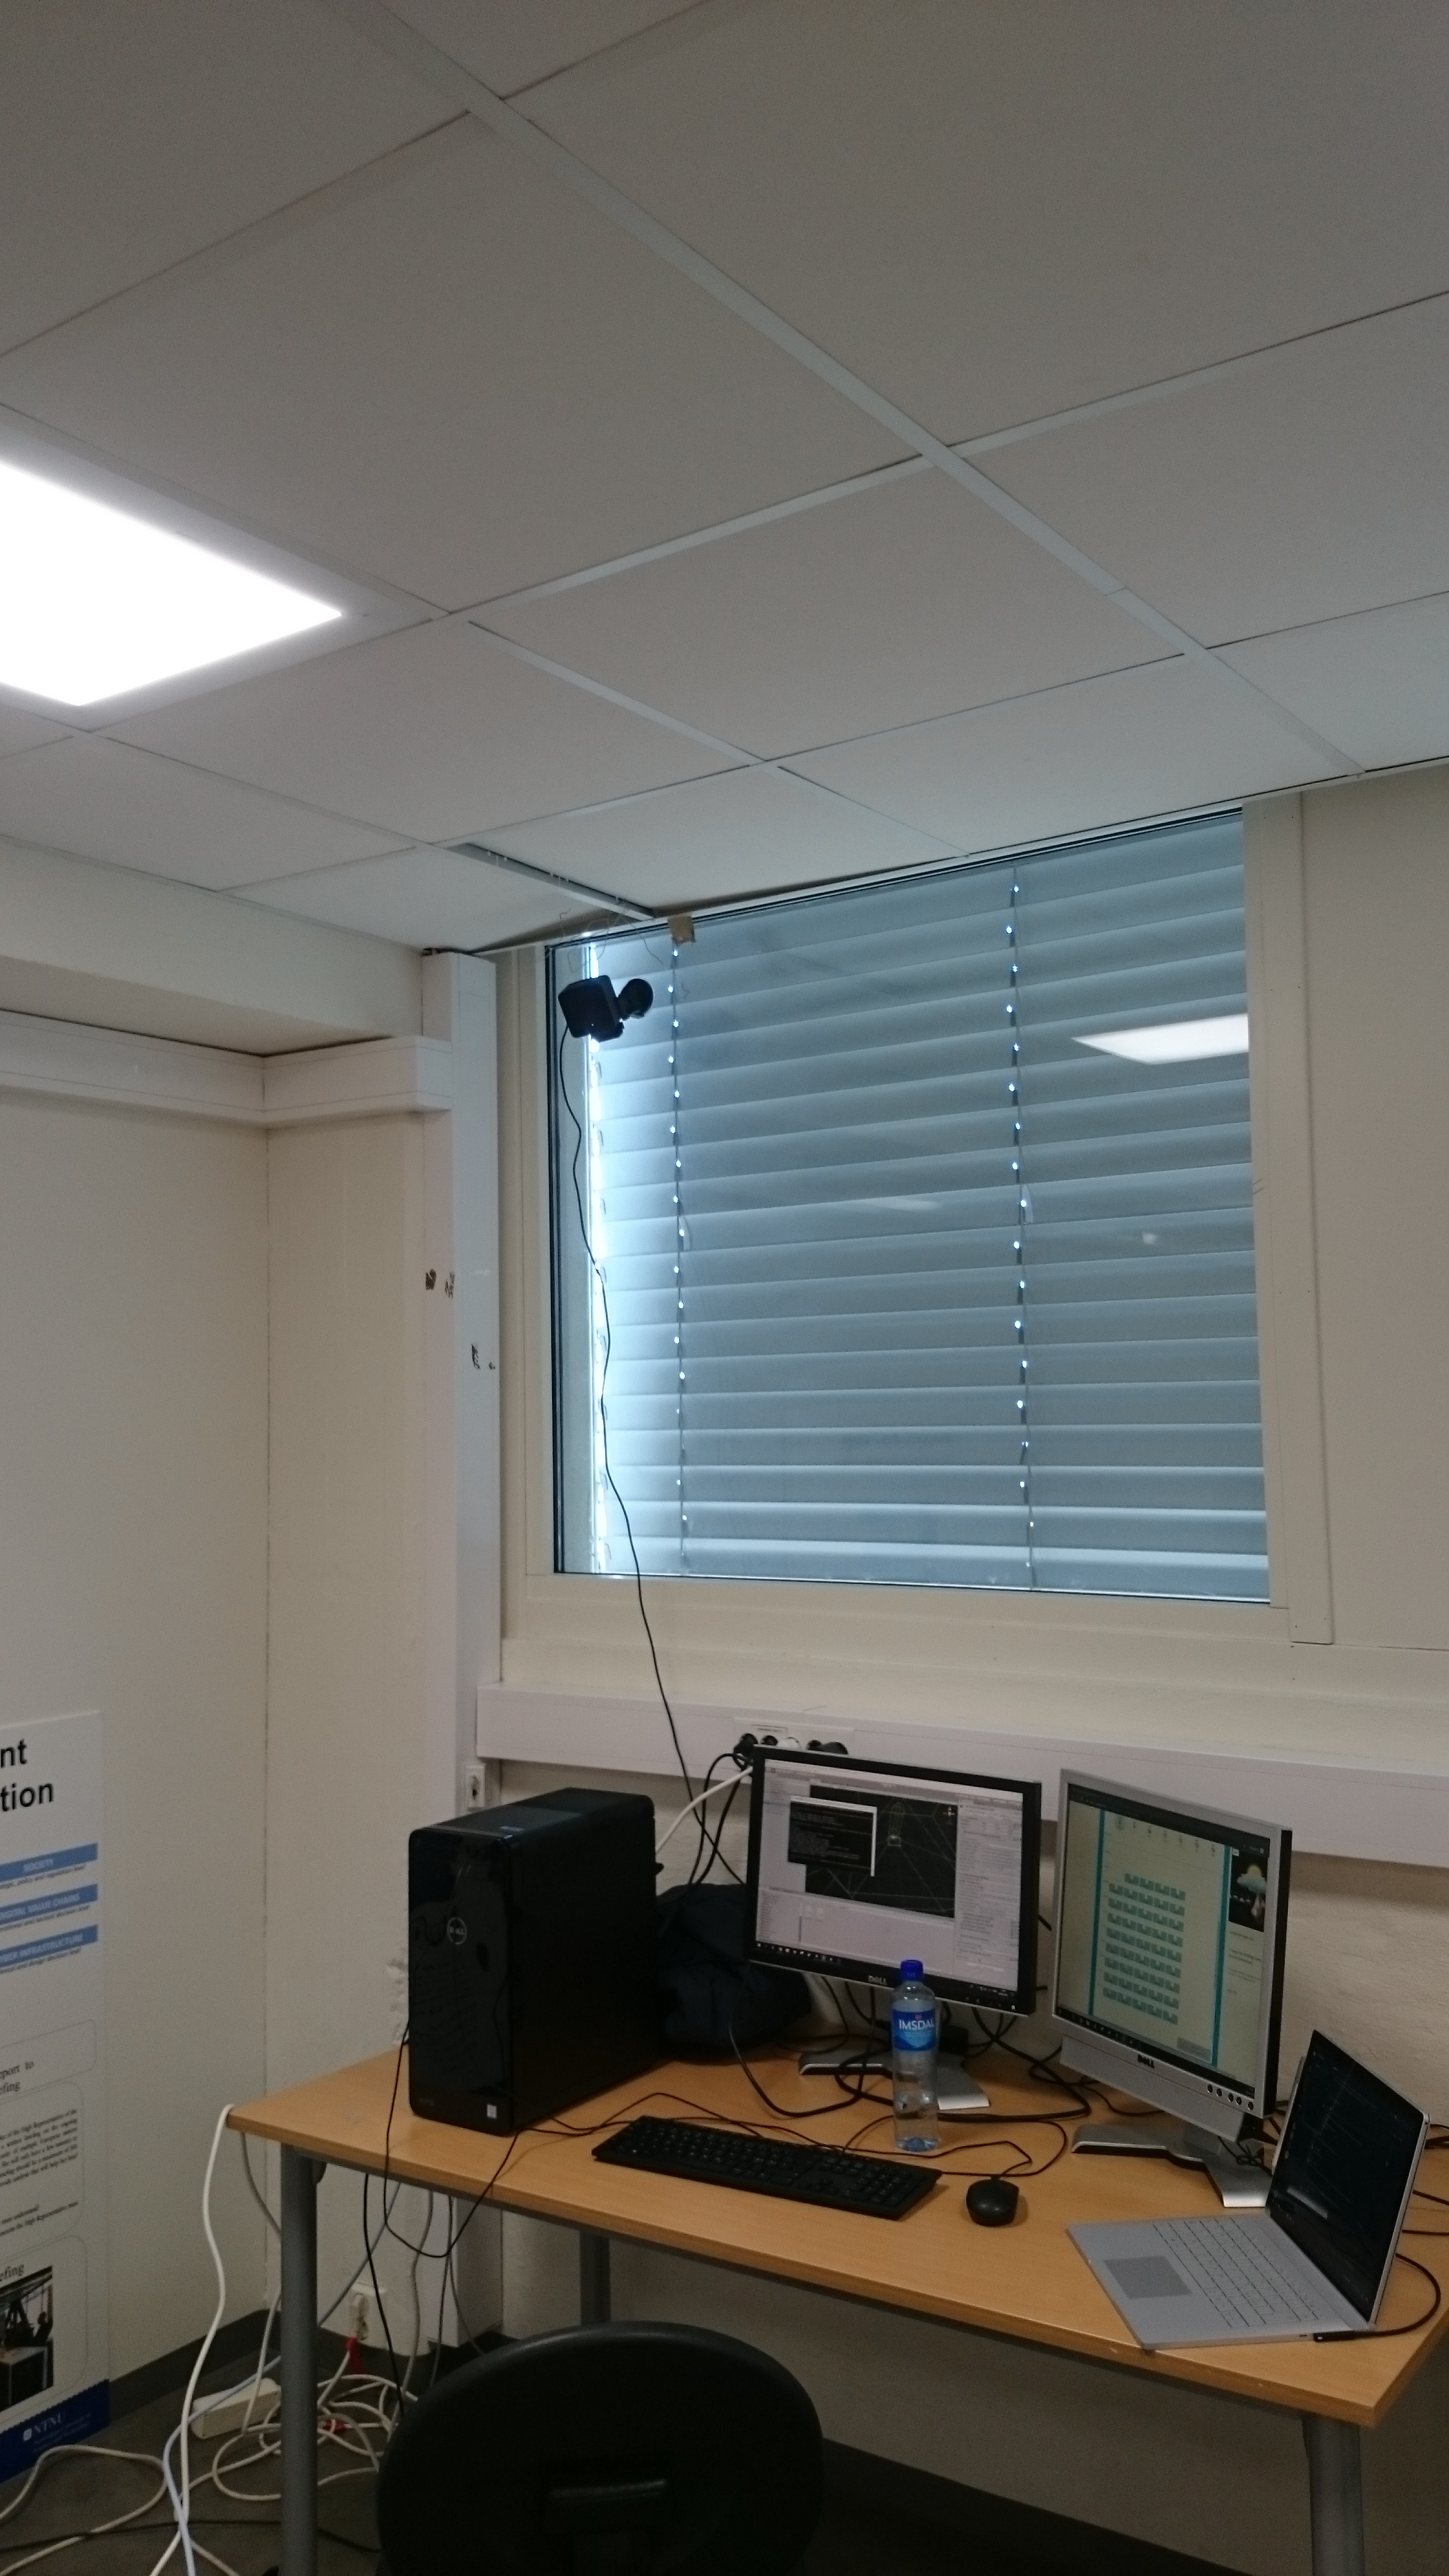
\includegraphics[width=0.25\textwidth]{figures/images/experiment2EnvironmentChanges.jpg}
    \caption[Changes in Experiment Environment for Experiment 2]{This image shows the alternative lighthouse setup that had to be made as the original ceiling mounted lighthouse disappeared before Experiment 2 started. Instead of a ceiling mounted solution, this setup makes use of a glass mounted lighthouse.}
    \label{fig:ex2changedLighthouse}
\end{figure}

There was a two week period between Experiment 1 and 2. During this time, one of the ceiling mounted HTC Vive lighthouses disappeared from the experiment setup with no trace or information on where it had gone. As such, it was necessary to set up a new lighthouse in a slightly different configuration. This configuration can be seen in Figure~\ref{fig:ex2changedLighthouse}. The disappearance of the original lighthouse was discovered on the weekend before the experiment started and as such, only limited amounts of room calibration testing was possible. This did create some calibration related problems for two participants. In particular, the reset boundaries became too wide for certain walls and resulted in resets not triggering. These calibration problems were fixed with a software workaround as soon as they were discovered and as such only affected two participants. The number of times the resets failed to trigger for each of these two were also noted down so they could be included with post-processing. 

\subsection{Participant Sample}
This section consists of information on how the participant sample was acquired, an overview of the demographics in the sample, what information participants were given and miscellaneous information. 
   
\subsubsection{Sampling Procedure}
The sampling procedure for Experiment 2 was the same as with Experiment 1. It consisted of advertisement by supervisors during lectures, information posters that were placed around campus, advertisement on the local NTNU Discord\footnote{\url{https://discordapp.com/}} server and general convenience sampling. It should be noted that participants who already took part in Experiment 1 were still allowed to participate in Experiment 2.

A variety of time slots were assigned to a doodle poll\footnote{\url{https://doodle.com/}} where participants could sign up with an alias for whatever time slot best fit their schedule. Participants were once again compensated with some chocolate for their time, albeit with less than in Experiment 1 since the amount of time spent for this experiment is shorter. In total, 15 participants signed up for Experiment 2, albeit only 13 of these showed up. These 13 were randomly distributed between the two conditions using the same Mersenne Twister library~\cite{MersenneTwisterLibraryLink} that previously has been mentioned throughout Chapter~\ref{chap:implementation}. This random distribution resulted in 7 participants for the control/S2C only condition and 6 in the experimental/S2C+AC2F condition. 

Acquiring participants for this experiment was generally more challenging as many students mentioned they already were fatigued by constantly taking part in the experiments of various master students. As such, a similar sample size to Experiment 1 was not possible to achieve within the same amount of sampling time. 

\subsubsection{Sample Demographics}
The sample itself primarily consisted of students within the age range of 18-24 years. Everyone in the sample identified as male and only one had to remove any optical corrections while participating. 11/13 participants had previous experience with redirected walking experiments due to a larger overlap from participants who already had taken part in Experiment 1. The general spread of VR experience is not quite as well distributed in this sample as compared to Experiment 1. This distribution can be seen in Figure~\ref{fig:ex2PriorVRExperience} where most participants answered with ''1'' and ''5'' on a Likert scale in terms of their prior VR experience.

\begin{figure}[tbph]
    \centering
    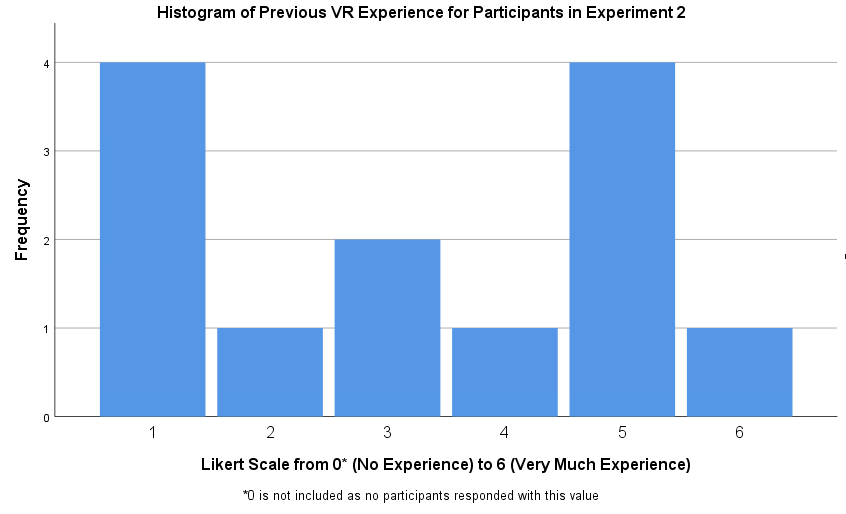
\includegraphics[width=0.75\textwidth]{figures/graphs/PriorVRExperienceExperiment2.png}
    \caption[Histogram on Prior VR Experience of Participants in Experiment 2]{This histogram shows the frequencies of what values participants provided in the demographics questionnaire of experiment 2 in terms of prior VR experience.}
    \label{fig:ex2PriorVRExperience}
\end{figure}

\subsubsection{Information and Consent}
In terms of information and consent, participants were given a sheet that was very similar to the one in Experiment 1. Both information/consent sheets can be seen in Appendix~\ref{app:informationconsent}. Participants were also given some oral information before playing through Ensemble Retriever. This was the same information which was given in Experiment 1, albeit without any mention of detection related information. 

The specific details and wording that was used for this oral information can be found in Section~\ref{sec:ex2information}.

\subsubsection{Miscellaneous Information and Issues}
As mentioned in Section~\ref{sec:ex2environmentchanges}, there were some problems related to the room calibration of the new lighthouse setup that had to be done. These problems affected participants 1 and 2 in particular, where participant 1 experienced one failed reset while participant 2 experienced two failed resets. Failed resets in this case are defined as the reset not triggering when it should. In order to avoid potential skewing of data, the number of times that the resets failed to trigger have been added to these participants during the data post-processing step which is mentioned in Section~\ref{sec:ex2postprocessing} and fully detailed in Section~\ref{sec:ex2postprocessingdetails}. 

\subsection{Changes in Ensemble Retriever Between Experiment 1 and 2}\label{sec:changesBetweenExperiments}
\begin{figure}[tbph]
    \centering
    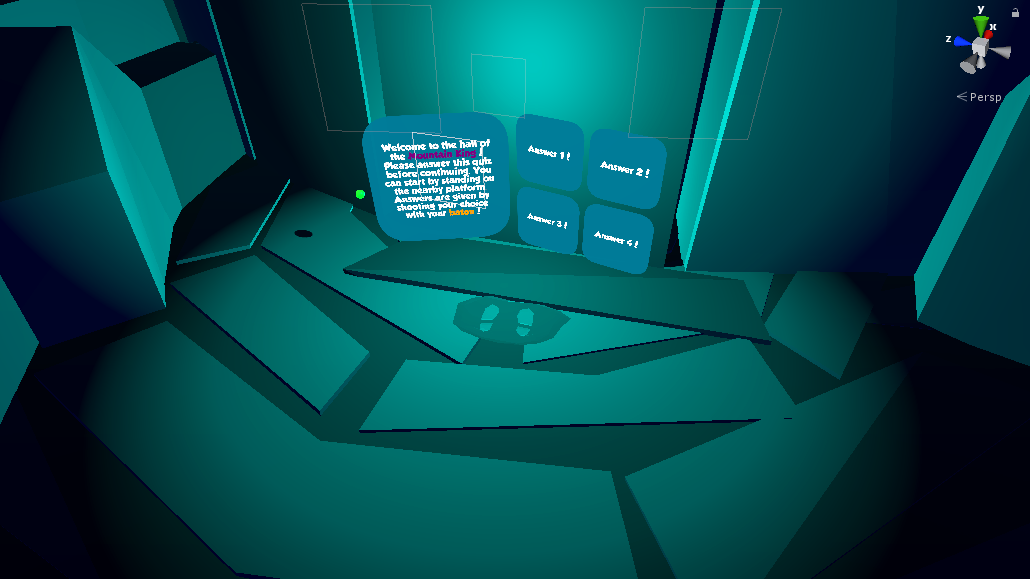
\includegraphics[width=0.5\textwidth]{figures/screenshots/HallOfTheMountainKingWithNewFloor.png}
    \caption[Screenshot of the ''Hall of The Mountain King'' Post Experiment 1]{This screenshot from the Unity scene view shows the updated ''Hall of The Mountain King'' after finishing Experiment 1. Some additional flooring has been added due to participant feedback to make traversal more natural.}
    \label{fig:mkhallWithFloor}
\end{figure}

A variety of things within Ensemble Retriever were changed between Experiment 1 and 2. The full change-log can be found in the project repository~\cite{projectRepository} by looking at the commit history, although this section will provide a summary of the changes that were implemented for Experiment 2. Some of these changes only apply when Experiment 2 is chosen as the active experiment in the software. These changes are marked with ''(EX2)'' while generic changes that apply to the entirety of Ensemble Retriever are marked with ''(ALL)''. The summary of changes are as follows:

\begin{itemize}
    \item Overall walking distance has been reduced to allow for a shorter experiment. (EX2)
    \item The health of the Mountain King has been cut in half to allow for a shorter experiment. (EX2)
    \item The tutorial does not provide any information on detection of redirection as this is only needed for Experiment 1. (EX2)
    \item S2C dampening is re-enabled as it no longer can affect the main focus of data collection. (EX2)
    \item The estimated detection thresholds from Experiment 1 are used as the redirection gains when playing. (EX2)
    \item An extra plane was added to the floor in the ''Hall of The Mountain King''. (ALL)
    \begin{itemize}
        \item This was changed due to feedback as participants mentioned it was awkward to walk between the large holes between the rocks in the floor. The difference can be seen by comparing Figure~\ref{fig:mkhallWithWall} and \ref{fig:mkhallWithFloor}.
    \end{itemize}
    \item The sound effect volume for absorbing projectiles has been increased to avoid being drowned out by the music. (ALL)
    \begin{itemize}
        \item This was changed due to participant feedback. Some participants noted that the music during the battle with the Mountain King was a bit high, so it was hard to clearly hear whenever they managed to absorb any projectiles. Hearing this audio is very useful when not directly looking in the direction the player is holding their hand. As such, the volume of the absorption sound effect was increased.
    \end{itemize}
    \item The floor in the ''Hall of The Mountain King'' has been better calibrated as the original calibration was lower than it should be, making some participants notice that their height was slightly inconsistent. (ALL)
    \item The buffer between reset and distractor triggers has been increased by 0.5m. This increase means that resets trigger 0.5m away from physical walls while distractors trigger at 1.5m instead of the previous 1.0m. (ALL)
    \begin{itemize}
        \item The reasoning behind this is that there were observations during Experiment 1 where participants would gradually increase their walking speed as they became more comfortable with the experience. Towards the end, walking speeds were fast enough that there would not be a large enough buffer between distractor and reset triggers, making both trigger instead of only the distractor. By increasing the buffer, the effective size of the walking space is slightly reduced, but should decrease the number of situations where resets trigger right after the distractor itself.  
    \end{itemize}
    \item Distractors like the Contrabass, Oboe and certain phases of the ''Mountain King'' have increased projectile speeds. (ALL)
    \begin{itemize}
        \item This was based on participant feedback for certain projectile attacks taking too long to reach the player, and thus being frustratingly slow. 
    \end{itemize}
    \item The hint providing fireflies in the environment now change colours after the player has visited them. (ALL)
    \begin{itemize}
        \item This was implemented due to participant feedback as a means to make it easier for somewhat disoriented players to see which of the fireflies they already had visited. 
    \end{itemize}
    \item The Distractor trigger magnitude cooldown has been decreased from 1.75m to 1.5m. (ALL)
    \begin{itemize}
        \item This was primarily done due to observations of situations where participants would walk a larger distance right as the death animation of a distractor starts. By the time it was finished and the cooldown initiated, the participant was almost at the bounds of the physical space, resulting in a reset instead of a distractor trigger. 
    \end{itemize}
\end{itemize}